% !TeX spellcheck = en_GB
\documentclass[11pt]{article}

\usepackage[type1]{libertine}
\usepackage[a4paper]{geometry}
\usepackage{amsmath, amsthm, amssymb} 
\usepackage{parskip}
\usepackage{tabularx}
\usepackage[english]{babel}
\usepackage{enumitem}
\usepackage{gensymb}
\usepackage{bm}
\usepackage{graphicx}
\graphicspath{{./graphics/}}
\usepackage[usenames, dvipsnames]{xcolor}
\usepackage{float}
\usepackage{wrapfig}
\usepackage{cancel}
\usepackage{multicol}
\usepackage{hyperref}
\usepackage{dashrule}
\usepackage{caption}
\usepackage[titletoc,title,toc,page]{appendix}

\newcommand{\nocontentsline}[3]{}
\newcommand{\tocless}[2]{\bgroup\let\addcontentsline=\nocontentsline#1{#2}\egroup}
\newcommand{\stoptocwriting}{%
	\addtocontents{toc}{\protect\setcounter{tocdepth}{-5}}}
\newcommand{\resumetocwriting}{%
	\addtocontents{toc}{\protect\setcounter{tocdepth}{\arabic{tocdepth}}}}

\usepackage{ccicons}

\renewcommand\thetable{\thesection-\arabic{table}}
\renewcommand\thefigure{\thesection-\arabic{figure}}

\usepackage{framed}
\colorlet{shadecolor}{yellow!35!} %BurntOrange!40 yellow!35! Black!20!

\usepackage{chngcntr}
\counterwithin{figure}{section}
\numberwithin{equation}{section}

\hypersetup{
	pdftitle={Lecture Notes - Newton's Laws of Motion},
	pdfauthor={Sun Yudong},
	bookmarksnumbered=true,
	bookmarksopen=true,
	bookmarksopenlevel=2,
	pdfstartview=Fit,
	pdfpagemode=UseOutlines,
	colorlinks=true,
	linkcolor=black,
	filecolor=magenta,      
	urlcolor=blue
}

\urlstyle{same}

\newenvironment{multicolFigure}
{\par\medskip\noindent\minipage{\linewidth}}
{\endminipage\par\medskip}
% https://tex.stackexchange.com/questions/12262/multicol-and-figures

\newcommand{\uvec}[1]{\boldsymbol{\hat{\textbf{#1}}}}
\newcommand{\solution}[1]{\textbf{Solution: } #1 \hspace{5mm}}

\title{Lecture Notes - Newton's Laws of Motion}
\author{Sun Yudong\\Hwa Chong Institution}
\date{March 3, 2018}

\begin{document}
	\maketitle
	\section*{Preface}
	These summary notes are meant to solely act as a guide for what the important and most poignant points that we went through in today and last week's lecture are. It is not meant to be an exhaustive revision resource, but can be your starting point as to what I think is important that needs to be understood. 
	
	\textbf{Even if you have attended the lecture, I recommend perusing through these notes}, because I have added some things that I missed out talking about in the lecture. This should also be useful in helping you consolidate the massive amount of content that was taught in the 2 to 2.5 hour lectures that we had. 
	
	Another aim of these notes is to provide you an overview (the big picture) of the topics and subtopics that we will be doing/have done, and why we are doing it. It is hoped that with this kind of big picture in mind, you can better appreciate Physics and the study of it. It would also then make your problem solving journey more motivating. 
	
	You are always welcome to ask questions if there are concepts you don't quite understand. Then I can also attempt to explain it in a better way to you. If you don't sound off, then I can't help you too. You may also not be the only one in class that has this query, and by discussing in class, I believe everyone can benefit. One good way to check if you understand the concepts is to try to solve questions. Once you get the topic, it would become increasingly more fun to solve questions, so don't give up.
	
	As this set of notes was rather rushed, there might be mistakes within the text. Do let me know if you encounter any. Thanks!
	
	We will explore more concepts on this topic when we eventually get to solving problems.
	
	For more in-depth information, please refer to the College Physics textbook. However, if you are comfortable with calculus, I strongly recommend using University Physics By Young and Freedman instead as your reference material.
	
	\textcolor[HTML]{aaaaaa}{\ccbysa}
	
	\pagebreak 
	\tableofcontents	
	\pagebreak
	\section{Introduction to Calculus Notation}
	Deriving from first principles, we want to investigate what is specifically the \textbf{the rate of change} of a certain property \textbf{at a specific given time.} In the example we used in the lecture, we used the graph/function of $S(t)$ to find what is the \textbf{rate of change of displacement with respect to time} i.e. the velocity. 
	
	In the example, we tried to find the velocity of an object undergoing constant acceleration by using looking at the change in displacement $x$ of the object at $t=t$ and $t=t+\varepsilon$. Mathematically speaking:
	\begin{equation}
		v=\lim\limits_{\varepsilon \,\rightarrow\, 0} \frac{x}{\varepsilon}=\lim\limits_{\Delta T \,\rightarrow\, 0} \frac{\Delta S}{\Delta T} =\frac{dS}{dt}
	\end{equation}
	where $\Delta T$ is your $\varepsilon$.
	
	By doing this derivation, we realize that we can derive the rules of differentiation. For more detailed information, look at \url{http://www.feynmanlectures.caltech.edu/I_08.html}. The opposite of this is integration:
	\begin{equation}
		\int_{0}^{t} v~dt = \int_{t=0}^{t=t} dS = S 
	\end{equation}
	
	The takeaway from this is to get familiar with the calculus notation and what it entails: $\frac{dy}{dx}$ is the \textbf{rate of change of y with respect x}, and integration is the opposite of differentiation, and we can use it to find the area under the graph.
	
	\vfill

	\hdashrule{\textwidth}{0.1mm}{1pt}
	
	The reason why I want you to be familiar with this notation and concept is that physics is ultimately most succinctly described with mathematics, and a lot of physics concepts involve rate of change, or the summation of certain functions over time. Being able to understand calculus would make it a lot easier to understand these topics. 
	
	You will formerly learn calculus in Secondary 4, and again more advanced calculus in JC, so don't worry if you do not yet know how to do mathematical manipulations/computations with calculus. Most importantly, I need you to understand the \textbf{concepts} behind it, and its corresponding notation and its implications. 
	
	\hdashrule{\textwidth}{0.1mm}{1pt}
	
	\pagebreak
	\section{Background to Dynamics}
	The aim of dynamics is to be able to find out \textbf{how we can affect motion}. To do this, we establish rules, and study how forces affect the motion of objects. 
	
	Before this chapter, we could not calculate and describe how a spring moves, and how I can make a ball fly across the room, but after this chapter, we will have the tools necessary to not just calculate and describe how a spring moves, but also how we can affect a ball's motion across the room, and even how the Earth moves around the Sun. 
	
	Together with the next chapter (Work, Energy, and Power), these concepts form the basis of all Mechanics. It is thus critical that you pay attention and spend extra time (if necessary) on these. 
	
	\section{The Laws of Motion}
	These laws set the basis of all force analysis. Newton's 1\textsuperscript{st} Law (N1L) lays out the basic condition for which the other laws apply. N2L tells us a mathematical description of how a force affects the motion of an object. N3L tells us that forces are interactions between 2 objects, and it always comes in pairs.
	
	Not lying here, but the wikipedia page (\url{en.wikipedia.org/wiki/Newton's_laws_of_motion}) provides a good overview of the newton's laws of motion, and its implications. Go read it if a textbook scares you. 
		\subsection{Newton's 1\textsuperscript{st} Law}
		\begin{shaded}
		 	In an inertial frame of reference, an object either remains at rest or continues to move at a constant velocity (\textbf{speed and direction}), unless acted upon by an external force.
		\end{shaded}
	
		This is also sometimes known as the law of inertia. Inertia is the resistance of an object to changes. The more massive an object, the harder it is change its motion. The quantitive measure of inertia is \textit{mass}.	Furthermore, if there are no net forces applied onto an object, then its motion does not alter (i.e. it undergoes \textit{uniform motion}). 
		
		This law sets up the idea of an inertial frame of reference. Newton's first and second laws are valid only in an inertial reference frame. \textbf{Any reference frame that is in uniform motion with respect to another inertial frame is also an inertial frame.} You can then disregard the reference inertial frame, and the laws of physics would apply similarly. 
		
		\pagebreak
		
		\subsection{Newton's 2\textsuperscript{nd} Law}
		\begin{shaded}
			In an inertial reference frame, the \textbf{vector sum} of the forces $\vec{F}$ on an object is equal to the mass $m$ of that object multiplied by the acceleration $\vec{a}$ of the object. (It is assumed here that the mass m is constant.)
			\begin{equation}
				\sum\vec{F} = m\vec{a} = m\frac{d\vec{v}}{dt} = \frac{d(m\vec{v})}{dt} = \frac{d\vec{p}}{dt}
			\end{equation}
		\end{shaded}
	
		This means that the effect of a force is proportional to the mass of the object. And in order to a achieve a certain acceleration, a proportional force must be applied. This law tells us how an applied force (bzw. applied forces) changes the motion of an object.
	
		There are a few assumptions in writing this down, but we shall examine limitations of this when we encounter them. The assumptions are:
		\begin{enumerate}
			\item The overall $m$ of the system does not change. If the mass is not constant, this law cannot be so simply applied.
			\item When 2 objects are together, their masses add.
		\end{enumerate}
		
		I have put some other information in Appendix \ref{appdx:n12l} so as not to clutter up these notes too much.
		
		\subsection{Newton's 3\textsuperscript{rd} Law}
		\begin{shaded}
		 	When one body exerts a force on a second body, the second body simultaneously exerts a force equal in magnitude and opposite in direction on the first body. Mathematically: 
		 	\begin{equation}
			 	\vec{F}_{\text{A on B}} = -\vec{F}_{\text{B on A}}
		 	\end{equation}
		\end{shaded}
		Forces always come in pairs because they are interactions between 2 objects. There are 3 properties of Action-Reaction pairs:
		\begin{enumerate}
			\item They are equal in magnitude and opposite in direction.
			\item They act on different objects.
			\item They are of the same type. 
		\end{enumerate}
	
	\pagebreak
	\section{Free-body Diagrams}
	There are 2 types of Free-Body Diagrams: 
	\begin{multicols}{2}
		\begin{multicolFigure}
				\centering
				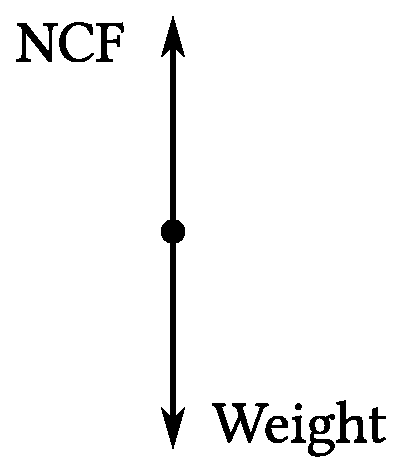
\includegraphics[height=3cm]{FBD_dot.eps}
		\end{multicolFigure}
		\begin{multicolFigure}
				\centering
				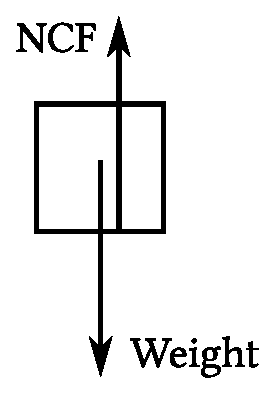
\includegraphics[height=3cm]{FBD_box.eps}
		\end{multicolFigure}
	\end{multicols}
	You might think that the boxed one is preferred in most situations, and you would be right, so long as you are dealing with day to day objects in the problems. Most of the time however, you would be dealing with things that we assume are point masses (e.g. in Gravitation, Nuclear Physics, ...), in which case the dot FBD would be much more useful. 
	
	Do get used to drawing diagrams like these as they are very useful in analysing the forces acting on a certain object. Only forces that act on the object can affect the object (duh). 
	
	When drawing free-body diagrams, it is poignant that we include \textit{\textbf{all}} the forces that are present. This way we would not forget when we do our analysis.
		\subsection{Proving angle on a slope}
		\begin{wrapfigure}{r}{5cm}
			\vspace{-0.7cm}
			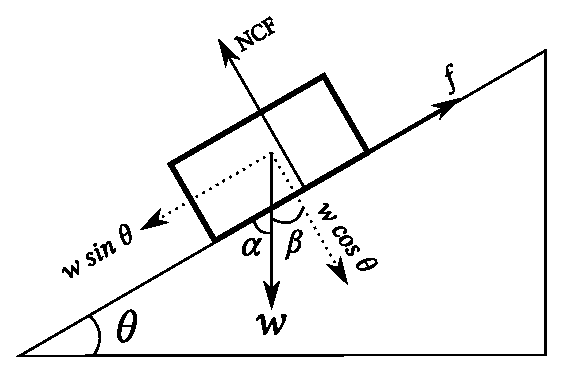
\includegraphics[width=5cm]{slope.eps}
			\caption{Slope}
			\label{fig:slope}
			\vspace{-1cm}
		\end{wrapfigure}
		Since $\alpha = 90\degree - \theta$, and $\beta = 90\degree - \alpha$, \\therefore $\beta = 90\degree - (90\degree - \theta) = \theta$.
		
		We usually resolve the force vectors along the incline of the slope because the motion is in that direction. If the forces are in equilibrium, we can also determine the magnitude of the other unknown forces that are present. 
	\section{Types of equilibrium}
		\begin{wrapfigure}{r}{3.5cm}
			\centering
			\vspace{-0.7cm}
			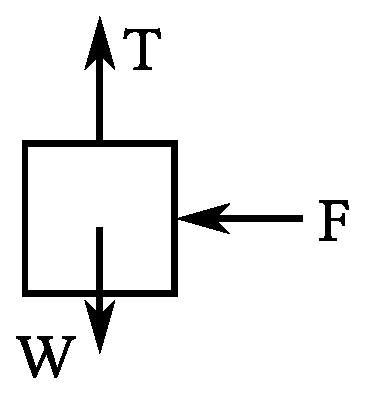
\includegraphics[width=2cm]{not_eqm.eps}
			\caption{An object not in equillibrium}
			\label{fig:not_eqm}
			\vspace{-0.5cm}
		\end{wrapfigure}
		Forces, just like in 2D-Kinemtics, can be resolved into independent orthogonal axes. \textbf{When an object is in equilibrium, it should be in equilibrium in all directions.}
		
		If it is not, then there should be a change in motion in the direction of the unbalanced force given by $\sum F=ma$. For example, in Figure \ref{fig:not_eqm}, the object should only be sliding to the right such that $a = F/m$.
		
		If this unbalanced force is only along one axis direction (as in Figure \ref{fig:not_eqm}), then the forces along the direction of the other axes should balance (i.e. $T = W$).
		\subsection{Translational}
		\begin{align*}
			\sum F = 0 ~~~~ a = 0 ~~~~ v = \text{constant}
		\end{align*}
		Dynamic equilibrium happens when $\sum F=0$, but $v \neq 0$. Static equilibrium happens when $\sum F=0$, and $v = 0$.
		\subsection{Rotational}
		\begin{align*}
		\sum F = 0 ~~~~ \sum \tau = 0 ~~~~ a = 0 ~~~~ v = \text{constant}
		\end{align*}
		where $\tau$ is torque. We will explore this more when we get to rotational motion.
%		\subsection{3-forces Systems}
%		For an object in equilibrium that has 3 forces acting on it, the lines of action of the 3 forces must coincide at a point. We will explore why this is the case when we look at rotational motion. B
	\section{Defining a System}
	When doing force analysis, it is very important to define the correct system. It can help us to simplify this problem a lot. \textbf{Only forces external to the system need to be considered}. \textbf{Internal forces cancel out} and cannot affect the motion of the system. Thus, if the problem doesn't need you to consider certain forces, it would be rather unwise to do extra work.
	
	This is best explained with an example. Consider the following train being pulled by a force $F$ that causes an overall acceleration of $a$:
	
	\begin{figure}[h]
		\centering
		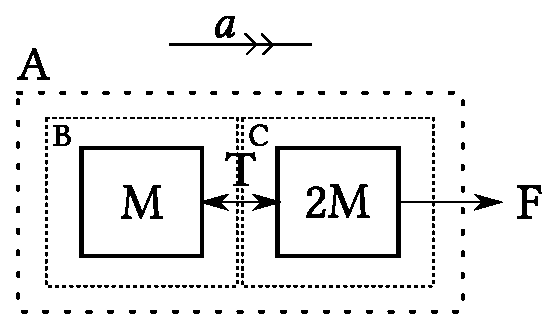
\includegraphics[width=5cm]{system.eps}
		\caption{A train with 2 carriages}
	\end{figure}
	
	If we want to find the tension $T$ of the connector between the 2 carriages, it would be helpful to just consider system $B$, as $T$ is the only external force acting on it. We can ignore all other forces. Since we know the acceleration of the block with mass $M$, we can apply $T=Ma$, and find $T$.
	
	Similarly, if we want to find the force $F$, it would be helpful to consider the whole system $A$. $T$ is an internal force, and so can be disregarded. The masses combine to give a total $3M$. Thus simply, $F = 3Ma$
	
	This kind of thinking can be very useful when it comes to pulley systems. By considering the entire setup as one system, we can easily find the acceleration $a$ of the entire system without needing to find out all the tensions involved.
	
	\section{Types of Forces}
		\subsection{Spring/Elastic}
		\begin{shaded}
			Force as a result of deformation in a spring (Hooke's Law):
				\begin{equation}
				\vec{F}=-k\vec{x}
				\end{equation}
				where $\vec{x}$ is the displacement of the spring from its equilibrium point.
		\end{shaded}
		Force is proportional to the displacement, and is \textbf{in the opposite direction} of the displacement.
		
		One interesting consequence of this is that, whether you deform the spring only on one end, or on both end, the force is \textbf{only dependent} on the displacement $\Delta x$:
		
		\begin{figure}[h]
			\centering
			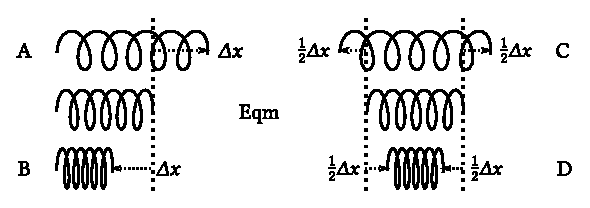
\includegraphics[height=2.5cm]{springs.eps}
			\caption{Springs stretched with amount $\Delta x$}
			\label{fig:springs}
		\end{figure}
	
		Due to the nature of springs, springs $A, B, C$ and $D$ all experience the same amount of force numerically, as they are all deformed to the same amount.
		
		If the spring is stretched beyond its ability to return back to its original equilibrium position, it will deform and the force $F$ will no longer follow Hooke's Law.
		
		\subsection{Tension}
		When we talk about tension in a string attached to objects, we usually assume a massless string so that there is 100\% of the force throughout the string. If the string is massive, a non-negligible force would then be required to balance the weight of the string.
		
		Key Characteristics:
		\begin{itemize}
			\item The force is the same throughout the string
			\item $\vec{F}_{A on B} = -\vec{F}_{B on A}$
		\end{itemize}
		\pagebreak
		To measure tension, we often use something called a spring balance: 
		
		\begin{figure}[h]
			\centering
			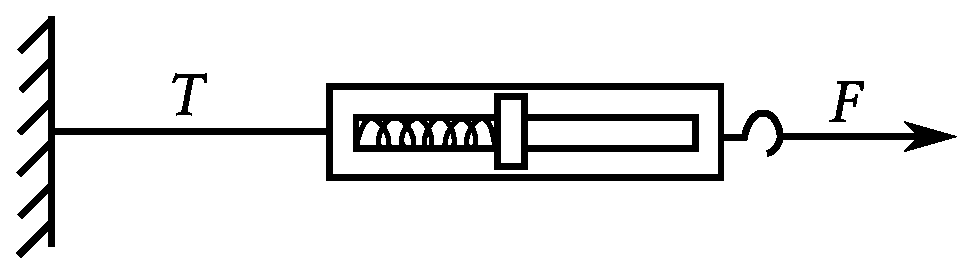
\includegraphics[height=1.5cm]{springbalance.eps}
			\caption{A spring balance measuring the tension $T$}
			\label{fig:springbalance}
		\end{figure}

		Since the whole system is in equilibrium, looking at the point where we connect the string to the balance, we realize that $T = F_{\text{spring}}$. The reading on the spring balance would thus exactly be the tension $T$.

			\subsubsection{Pulleys}
			Through tension of a massless string, pulleys change the direction of a force without loss. 
		
			\begin{multicols}{2}
				\begin{multicolFigure}
					\centering
					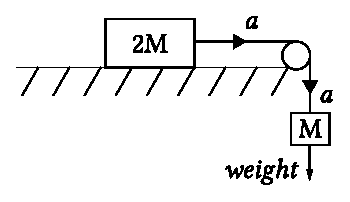
\includegraphics[height=2.9cm]{pulley.eps}
					\captionof{figure}{Pulley system on a table}
					\label{fig:pulley-table}
				\end{multicolFigure}
				\begin{multicolFigure}
					\centering
					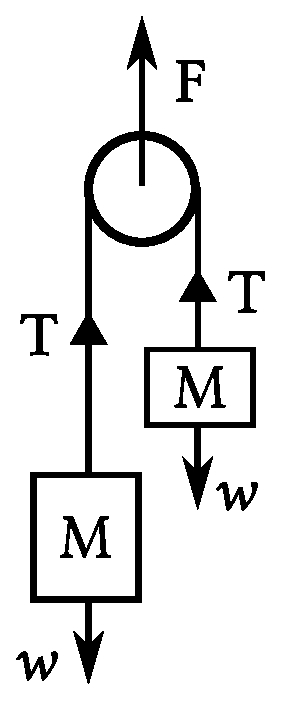
\includegraphics[height=2.9cm]{pulley2.eps}
					\captionof{figure}{Hanging pulley system}
					\label{fig:pulley-hang}
				\end{multicolFigure}
			\end{multicols}
		
			\begin{wrapfigure}{r}{3.5cm}
				\centering
				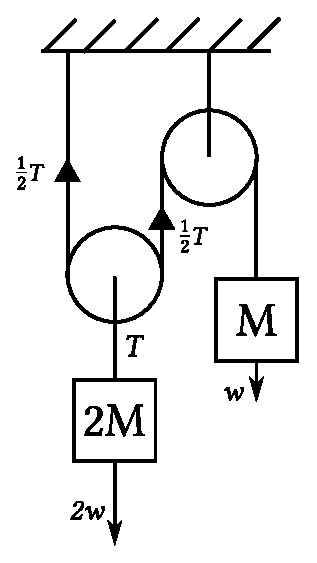
\includegraphics[width=2.5cm]{movablepulley.eps}
				\caption{A system with a movable pulley}
				\label{fig:movablepulley}
				\vspace{-1cm}
			\end{wrapfigure}
		
			Most of these I'm sure you already intuitively understand.
			
			In Figure \ref{fig:pulley-table}, the only force pulling the system of 2 masses is the weight of mass $M$. The direction of it changes and accelerates the entire system of $M+2M$. 
			
			In Figure \ref{fig:pulley-hang}, the weight of the 2 masses are balanced out by force F, but looking individually, the weight of the 2 masses are balanced out by each other so that no particular side accelerates.
			
			Due to the properties of pulleys, we can also make machines with them. As we can see in Figure \ref{fig:movablepulley}, the movable pulley decreases the effort required to lift the weight of the $2M$ mass. Compared to the system in Figure \ref{fig:pulley-hang}, it reduces the effort by half.
			
			In all of these examples, we assume all surfaces are frictionless.
			
		\pagebreak
		\subsection{Contact Forces}
		When 2 surfaces come into contact, there will always be contact forces. This force can be broken down into 2 components:
		\begin{itemize}
			\item Normal Contact Force (Normal to the surface)
			\item Friction (along the surface)
		\end{itemize}
		The sum of these 2 component forces add up to the contact force. 
			\subsubsection{Friction}
			There are 2 types of friction:
			\begin{itemize}
					\item Static Friction ($f_s \leq \mu_s N$)
					\item Kinetic Friction ($f_k \leq \mu_k N$) 
			\end{itemize}
			where N is the magnitude of the normal contact force. It has been observed that $f_k < f_s$.

			As friction always opposes motion, the direction of friction will always be pointing in the opposite direction of motion, whether the object is already in motion, or is still stationary (you can also think of it as supposed motion). 

			Due to the nature of friction, the value of friction is not set. Only a maximum can be obtained using the above formula. Usually, the magnitude of friction is obtained by means of analysing the forces involved in the problem. 
		\subsection{Weight and Weightlessness}
		Weight is the force of gravity on a massive object. It is proportional to mass in the following manner:
		\begin{equation}
			W = mg ~~~\Leftrightarrow~~~F=ma
		\end{equation}
		where $g$ is the local gravitational acceleration at that point in space (whether it is the moon or the Earth or somewhere else).

		Usually, we experience and measure weight by measuring the normal contact force between the surface and the object. This is how we most commonly measure weight. So if we reduce the normal contact force to zero, we can be considered ``weightless".
			\subsubsection{Difference between Mass and Weight}
			Mass is the measure of inertia of an object. It tells us how massive the object is, how much matter is inside the object. Weight is the force experienced by a massive object in a gravitational field. 
			\subsubsection{``Elevator Problems"}
			\begin{wrapfigure}{r}{4.2cm}
				\centering
				\vspace{-0.7cm}
				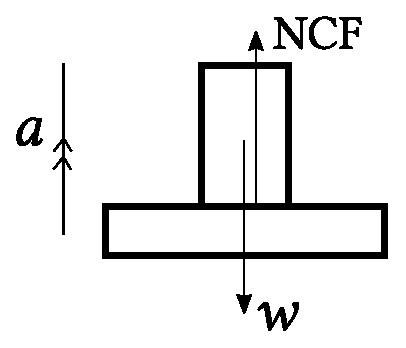
\includegraphics[width=4cm]{elevator.eps}
				\caption{An person in an elevator}
				\label{fig:elevator}
				\vspace{-0.7cm}
			\end{wrapfigure}

			When a vehicle is undergoing acceleration, we might feel changes to the \textbf{apparent weight} of a person. This disappears once the vehicle is at constant velocity. 

			To explain why, we look specifically at a person in a lift, standing on a balance (Figure \ref{fig:elevator}). Since there is an overall acceleration of the man, we notice that:
			\begin{align*}
				\sum F = N - w &= ma \\
				N &= ma + w 
			\end{align*}
			Since we measure weight by measuring the normal contact force, we can see that the normal contact force has now increased in magnitude, resulting in the feeling of being heavier when the elevator is accelerating.

		\pagebreak
		\subsection{Fluid Mechanics I}
			This part is from Chapter 12 of your textbook. 
			\vspace{-0.3cm}
			\subsubsection{Pressure}
			The force that a fluid exerts is always perpendicular to the surface on which it acts on.  However, during the analysis of fluids, we often examine the pressure instead of the force:
			\begin{equation}
			P=\frac{F}{A} ~~~ \text{or force per unit area}
			\end{equation}					
			We often measure pressure using a barometer by looking at the pressure differences between 2 environment. The standard unit is the Pascal \textit{(Pa)}. $1$ atm $= 101325$ Pa $= 760$ mmHg.
			\subsubsection{Fluid Pressure}
			\begin{shaded}
				The pressure at any given point of a non-moving (static) fluid is called the \textbf{hydrostatic pressure}:
				\begin{equation}
					\label{eqn:fluidpressure}
					P = P_0 + \rho g h 
					%\left( = \frac{F}{A} = \frac{mg}{A} = \frac{\rho Ahg}{A} \right) 
				\end{equation}
				where $\rho$ is the density of the fluid and $P_0$ is the pressure at the surface of the fluid. This pressure is due to the weight of the fluid column above that point.
			\end{shaded}
			Notice that the pressure is the same at any 2 points at the same level in the fluid. The shape of the container does not matter.  \textbf{It only depends on the depth.}
			
			% Intuitively, this is because the liquid, when static, must be in equilibrium. This means that should the water level increase in one part of the container, the increase in pressure would cause the water level in the other part of the container to rise as well so that the pressure at the bottom of the container is the same. This balance means that \textbf{only if the pressure is the same at a particular point from all directions, the liquid cannot be in equilibrium}.
			
			Discussions of liquid pressure usually refer to the pressure without regard to the normally ever-present atmospheric pressure. In fact, when we usually measure pressure, we are interested in the \textbf{Gauge Pressure}, which is the $\Delta P = P_{\text{absolute}} - P_0$. 
			
			Refer to Appendix \ref{appdx:fluidpressure} for more information. 
			\subsubsection{Pascal's Principle}
			Consequently, from equation \ref{eqn:fluidpressure}, if we increase the pressure $P_0$ at the top surface, the pressure at any depth increases by exactly that amount. This observation is known as Pascal's Principle:
			\begin{shaded}
				A change in pressure at any point in an enclosed fluid at rest is transmitted undiminished to all points in the fluid. Mathematically,
				\begin{equation}
				\Delta P = \rho g \Delta h
				\end{equation}
			\end{shaded}
			Applying this law, we can also build hydraulic lifts. Refer to Appendix \ref{appdx:hydraulic} for more information. 
			\subsubsection{Upthrust and Buoyancy --- Archimedes Principle}
			\begin{shaded}
				When a body is completely or partially immersed in a fluid, \textbf{the fluid exerts an upward force on the body equal to the weight of the fluid displaced by the body}. Mathematically,
				\begin{equation}
					\begin{aligned}
					\label{eqn:upthrust}
					U &= \rho_{_{\text{fluid}}} \cdot V_{_{\text{displaced}}} \cdot g \\
					U &= \rho V\!g
					\end{aligned}
				\end{equation}
				Upthrust is present whether the object sinks ($w > U$) or floats ($w \leq U$). An object floats in equilibrium when
				\begin{equation}
					\begin{aligned}
					U &= w  \\
					\rho_{_{\text{fluid}}} V_{_{\text{displaced}}} g &= m_{_{\text{object}}}g
					\end{aligned}
				\end{equation}
				This is the case whether the object is fully or partially submerged.
			\end{shaded} 
			Note that the $V_{\text{displaced}}$ is \textbf{the volume of fluid displaced}, and not necessarily the volume of the object. The derivation of \eqref{eqn:upthrust} from \eqref{eqn:fluidpressure} can be found in Appendix \ref{appdx:upthrust}.
			
			Notice that no matter how heavy an object is, so long as it can displace enough fluid, it will experience an upthrust enough to keep it afloat.
			
			Since there is a buoyant force acting on the submerged object, the object also exerts a reaction force on the water equivalent in magnitude to the buoyant force, but pointing in the opposite direction to the upthrust. 
			\subsubsection{Viscosity and Fluid Resistance}
			Viscosity is the internal friction in a fluid. Viscous fluids resist the relative motion of immersed objects through them as well as to the motion of one portion of a fluid to another. The strength of the viscous resisting forces is characterized by the \textit{coefficient of viscosity} $\eta$ (eta). An example of a very viscous fluid is honey.
			
			The concept of viscosity is important to the analysis of resistive forces in a fluid when an object moves through it.
			
			Suppose we have a sphere of radius $r$ moving through a fluid of viscosity $\eta$ with velocity $v$. We assume that $v$ is sufficiently small so that the flow of fluid is \textbf{not turbulent}\footnote{For turbulent flow, the resistive drag force is typically approximately proportional to $v^2$}. 
			
			\vfill
			\begin{shaded}
			The resistive force $F$ that this sphere experiences as a result of this motion through a \textbf{laminar fluid flow} is proportional to $v$, more specifically: 			
				\begin{equation}
				F_r = 6\pi \eta r v \implies F_r \propto v
				\end{equation}
				This is called \textbf{Stoke's Law}.
			\end{shaded}
			\vfill
			\pagebreak
			
			With this, we can now analyse \textbf{terminal velocity $v_0$} of a sphere falling through a fluid (e.g. Air):
			\begin{align*}
				\sum F = F_r - w &= 0 \\
				F_r &= mg \\
				6\pi \eta r v_0 &= \left(\frac{4}{3}\pi r^3 \rho \right)g
			\end{align*}
			or,
			\begin{equation*}
				v_0 = \frac{2}{9} \left(\frac{r^2\rho g}{\eta}\right)
			\end{equation*}
			
			Practically, you can only apply this to a small number of situations. Most situations in everyday life (e.g. a car driving down a highway) involve chaotic behaviours (e.g. turbulent flow) that would make such analysis very difficult\footnote{Turbulence poses some profound questions for theoretical physics. How is it that a system that obeys well-defined and supposedly deterministic physical laws can have unpredictable, chaotic behaviours? \par There are no simple answers, and indeed the study of chaotic behavious in deterministic systems is still a highly active field of research.}.
			
			\vfill
			\hdashrule{\textwidth}{0.1mm}{1pt}
			
			It might be useful to know that the way we have examined things in this section is not yet very rigorous. We will examine the concepts again in greater detail when we go through Fluid Mechanics II. 
			\vspace{-0.2cm}
			
			\hdashrule{\textwidth}{0.1mm}{1pt}
			\vfill
		\newpage
		
		\begin{appendices}
			\stoptocwriting
			\section{Newton's 1\textsuperscript{st} and 2\textsuperscript{nd} Law}
			\label{appdx:n12l}
			Looking at the mathematical description:
			
			\begin{equation}
			\sum\vec{F} = m\vec{a} = m\frac{d\vec{v}}{dt} = \frac{d(m\vec{v})}{dt} = \frac{d\vec{p}}{dt}
			\end{equation}
			
			you can realize that Newton's second Law is consistent with the first law: 
			\begin{equation}
			\sum \vec{F} = 0 \Leftrightarrow \frac{d\vec{v}}{dt} = 0
			\end{equation}
			This means that if there is no net external force on an object, then the object must not have a change in its velocity; and conversely, if the object is not experiencing a change in its velocity, then there must be no net external force on the object. 
			
			It should be noted that velocity here is a vector and involves not just the speed, but also the direction. Hence, if there is a change in the direction of the velocity, there must be an acceleration (we will explore this later in circular motion). 
			
			The $p$ in the 2\textsuperscript{nd} part of the equation is \textit{\textbf{momentum}}. We will explore the concepts of momentum in a later chapter. For a massive particle (a particle with mass), it is numerically equal to $m\vec{v}$. If you are dealing with the force exerted on/by massless particles that have momentum, but no mass (e.g. photons), then we have to use N2L written in this form.
			\pagebreak
			\section{Fluid Pressure}
			\label{appdx:fluidpressure}
			The pressure at any given point of a non-moving (static) fluid is called the \textbf{hydrostatic pressure}:
			\begin{equation}
				\label{eqn:appdx:fluidpressure}
				P = P_0 + \rho g h 
			\end{equation}
			where $\rho$ is the density of the fluid and $P_0$ is the pressure at the surface of the fluid. This pressure is due to the weight of the fluid column above that point.
			
			To derive this, we first look at a certain point in a fluid. The force on the horizontal plane of this point cancel out, and so we are only left with the vertical components of this force. Since the liquid is in equilibrium, then it follow that the point would also be in equilibrium:
			\begin{align*}
				F &= w = mg = (\rho V) g = (\rho Ah)g \\
				P &= \frac{F}{A} = \frac{\rho \cancel{A}hg}{\cancel{A}} = \rho gh
			\end{align*}
			
			Atmospheric pressure pressing on the surface of a liquid must be taken into account when trying to discover the total pressure acting on a liquid. The total pressure of a liquid, then, is 
			\begin{equation*}
				\rho gh + P_{\text{atm}}
			\end{equation*}
			In general form, where the surface of the water is not interfacing normal atmospheric pressure, we obtain \eqref{eqn:appdx:fluidpressure}.
			
			For a more rigorous derivation of fluid pressure, please refer to College Physics pp. 410-411.
			
			When this distinction is important, the term \textit{total pressure} is used. Otherwise, discussions of liquid pressure refer to pressure without regard to the normally ever-present atmospheric pressure.
			
			\subsection{Measuring Pressure}
			
			\begin{wrapfigure}{r}{5.2cm}
				\centering
				\vspace{-0.7cm}
				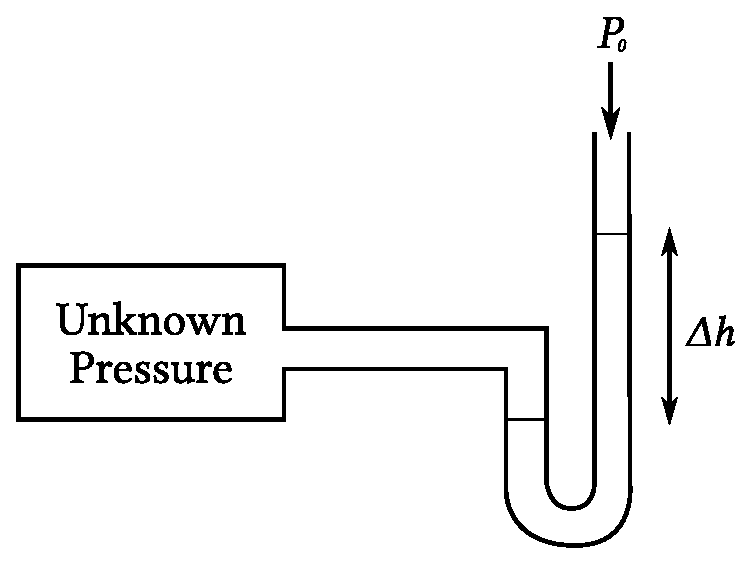
\includegraphics[width=4.5cm]{barometer.eps}
				\caption{A manometer that uses millimetres of Mercury as its units of measurement}
				\vspace{-0.5cm}
			\end{wrapfigure}
		
			To measure pressure, we often use devices like barometers. For liquid manometer, it works on the same concepts that govern all liquids. By observing the difference in liquid level across a u-tube, we can find the difference in pressure, thereby obtaining the gauge pressure:
			\begin{align*}
				P + \rho g h_1 &= P_0 + \rho g h_2 \\
				P - P_0 &= \rho g \Delta h
			\end{align*}			
			Since the pressure at the bottom of the tube are measured at the same level from the left and right, and so much be equal.
			
			Note that we prefer to use \textit{Pa} instead of \textit{mmHg} as the unit of measurement as \textit{mmHg} depends on the density of mercury (which varies with temperature) and g (which varies with location).
			
			\pagebreak
			\section{Hydraulic Lifts}
			\label{appdx:hydraulic}
			\begin{wrapfigure}{r}{5cm}				
				\centering
				\vspace{-0.7cm}
				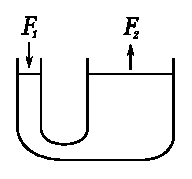
\includegraphics[width=3cm]{hydraulic.eps}
				\caption{A hydraulic lift}
				\label{fig:appdx:hydraulic}
				\vspace{-0.5cm}
			\end{wrapfigure}
			A hydraulic lift (Figure \ref{fig:appdx:hydraulic}) illustrates Pascal's principle. When a piston exerts a small force $F_1$, the applied pressure $p=F_1/A_1$ is transmitted throughout the liquid to the other larger piston. Since the applied pressure is the same in both the left and right side, we obtain:
			\begin{equation}
				p = \frac{F_1}{A_1} = \frac{F_2}{A_2} \implies F_2 = \left(\frac{A_2}{A_1}\right) F_1
			\end{equation}
			As a result, the output force $F_1$ is greatly amplified by the ratio $A_2/A_1$ to give a much larger $F_2$.
			
			\section{Derivation of Upthrust}
			\label{appdx:upthrust}
			\begin{wrapfigure}{r}{5cm}				
				\centering
				\vspace{-0.7cm}
				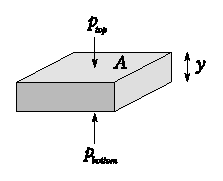
\includegraphics[width=4cm]{upthrust.eps}
				\caption{A hydraulic lift}
				\label{fig:appdx:upthrust}
				\vspace{-0.5cm}
			\end{wrapfigure}
			Let's take an arbitrary object submerged in water at depth $h$ from the top (Figure \ref{fig:appdx:upthrust}). The forces on the side of the object cancel out, hence we can simply look at the vertical components:
			\begin{align*}
				\sum F_y &= F_{\text{bottom}} - F_{\text{top}} \\
				&= A(P_{\text{bottom}} - P_{\text{top}}) \\
				&= A\rho g((h+y) - h) \\
				&= \rho (Ay)g \\
				&= \rho V \! g
			\end{align*}
			Note that here the $\rho$ is the density of the fluid. Hence, the $\rho V\!g$ obtained is the weight of the fluid displaced.
			\resumetocwriting
		\end{appendices}
		
\end{document}